\documentclass[12pt,a4paper]{article}

% ============================================================================
% PREAMBULO
% ============================================================================

\usepackage[
    top=3cm,
    bottom=2cm,
    left=3cm,
    right=2cm
]{geometry}

\usepackage{setspace}
\onehalfspacing

\usepackage{graphicx}
\usepackage{float}
\usepackage{hyperref}
\usepackage{listings}
\usepackage{xcolor}
\usepackage{fancyhdr}

% Cores para código
\definecolor{backcolour}{rgb}{0.95,.95,0.92}

\lstset{
    backgroundcolor=\color{backcolour},
    basicstyle=\ttfamily\small,
    breaklines=true,
    captionpos=b,
    numbers=left,
    numbersep=5pt,
    tabsize=2,
    language=bash
}

\hypersetup{
    colorlinks=true,
    linkcolor=blue,
}

\pagestyle{fancy}
\fancyhf{}
\rhead{CTF - Detetives Criptográficos}
\lhead{UFSC}
\cfoot{\thepage}
\setlength{\headheight}{15pt}

% ============================================================================
% DOCUMENTO
% ============================================================================

\begin{document}

% ============================================================================
% CAPA SIMPLES
% ============================================================================

\begin{titlepage}
    \centering
    \vspace*{3cm}
    
    {\Large \textbf{UNIVERSIDADE FEDERAL DE SANTA CATARINA}} \\
    \vspace{1cm}
    {\Large Segurança da Computação} \\
    
    \vspace{3cm}
    
    {\LARGE \textbf{CTF - Detetives Criptográficos}} \\
    \vspace{0.5cm}
    {\large Análise de Segurança e Exploração}
    
    \vspace{4cm}
    
    {\large Aluno: Artur Luiz Rizzato Toru Soda}
    
    \vspace{0.5cm}
    {\large Matrícula: 22200349}
    
    \vspace{0.5cm}
    {\large Data: 26/05/2026}
    
    \vspace{0.5cm}
    {\large Professores: Profa. Thaís Bardini Idalino e \\ Prof. Jean Everson Martina}

    \vspace{\fill}
    
    Florianópolis, SC -- 2026
    
\end{titlepage}

% ============================================================================
% ÍNDICE
% ============================================================================

\tableofcontents
\newpage

% ============================================================================
% INTRODUCAO
% ============================================================================

\section{Introdução}

Este relatório foi escrito no formato de registro técnico sequencial, acompanhando a resolução do desafio passo a passo. Em cada etapa, foi documentado:

\begin{itemize}
    \item o que foi possível extrair como informação útil naquele momento;
    \item a metodologia e o vetor de ataque com comandos reproduzíveis;
    \item o mapeamento das primitivas criptográficas envolvidas e a forma de contorno;
    \item as evidências visuais de comprometimento (capturas de terminal).
\end{itemize}

Com isso, a narrativa permanece fluida e cronológica, desde a inspeção inicial do \texttt{secret.txt} até a aprovação final do documento forjado pelo \texttt{verificador}.

\subsection{Objetivo técnico e critério de sucesso}

O objetivo operacional deste trabalho foi reproduzir, de forma técnica e auditável, um fluxo de comprometimento da confiança do sistema alvo sem quebra matemática das primitivas criptográficas principais.
O critério de sucesso adotado foi a aprovação, pelo \texttt{verificador}, de um documento forjado e assinado com identidade não legítima, acompanhada de evidências de terminal e mapeamento das primitivas envolvidas.

% ============================================================================
% PASSO 1: DECODIFICAÇÃO
% ============================================================================

\section{Passo 1: Decodificação do Secret.txt}

\subsection{Informações extraídas neste passo}

Da apresentação, sabemos que o \texttt{secret.txt} possui exatamente 64 caracteres ASCII (512 bits) e representa a pista inicial para as próximas etapas.

\subsection{Metodologia e Vetor de Ataque (Reprodutibilidade)}

\subsubsection{Análise Inicial}

O arquivo \texttt{secret.txt} contém:

\begin{lstlisting}
Teve$ywev$s$zivmjmgehsv$gsrwypxi
$ew$mrxvy??iw0$oAwikvihs$EIWcGFG
\end{lstlisting}

Características:
\begin{itemize}
    \item Tamanho: 64 caracteres ASCII (512 bits)
    \item Formato: Texto cifrado em duas linhas
    \item Tipo de cifra: Variação de Caesar Cipher
\end{itemize}

\subsubsection{Comandos executados}

Para quebrar a cifra, utilizamos força bruta testando todos os shifts possíveis (0-255):

\begin{lstlisting}[caption=Script Python para decodificar]
cifrado = "Teve$ywev$s$zivmjmgehsv$gsrwypxi$ew$mrxvy??iw0$oAwikvihs$EIWcGFG"

for shift in range(1, 256):
    decifrado = ""
    for char in cifrado:
        novo_valor = ord(char) - shift
        if novo_valor < 0:
            novo_valor += 256
        decifrado += chr(novo_valor)

    texto = decifrado.lower()
    if all(x in texto for x in ["para usar", "verificador", "consulte", "k=segredo"]):
        print(f"[SHIFT {shift}] {decifrado}")
\end{lstlisting}

\subsubsection{Resultado observado}

\begin{figure}[H]
    \centering
    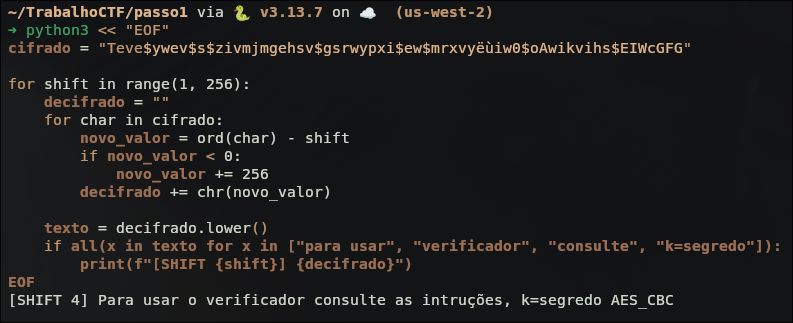
\includegraphics[width=1.0\textwidth]{screenshots/passo1_decodificacao.png}
    \caption{Output do script mostrando a decodificação bem-sucedida}
    \label{fig:passo1}
\end{figure}

Chave extraída: \texttt{segredo}

\subsection{Mapeamento de Primitivas Criptográficas}

Neste passo, a primitiva principal foi uma cifra de substituição do tipo Caesar sobre bytes ASCII.
O propósito arquitetural era esconder a senha do próximo estágio sem expor o segredo em texto claro.
O contorno foi feito por força bruta completa no espaço de deslocamentos (0--255), com validação por legibilidade do texto em português e identificação de padrão de segredo.


% ============================================================================
% PASSO 2: DESCRIPTOGRAFIA
% ============================================================================

\section{Passo 2: Descriptografia do Arquivo IUVA}

\subsection{Informações extraídas neste passo}

A mensagem decodificada no Passo 1 indica a chave \texttt{segredo} e o uso de \texttt{AES\_CBC}. Isso direciona diretamente a tentativa de decriptação do arquivo \texttt{IUVA}.

\subsection{Metodologia e Vetor de Ataque (Reprodutibilidade)}

\subsubsection{Análise Inicial}

O arquivo IUVA é um binário criptografado originalmente em formato PDF, usando criptografia simétrica moderna (OpenSSL).

\subsubsection{Comandos executados}

\begin{lstlisting}[caption=Descriptografar com OpenSSL]
openssl enc -d -aes-256-cbc -a -in IUVA -out documento.pdf \
  -pass pass:"segredo" -pbkdf2

file documento.pdf

head -c 10 documento.pdf  
\end{lstlisting}

\subsubsection{Resultado observado}

\begin{figure}[H]
    \centering
    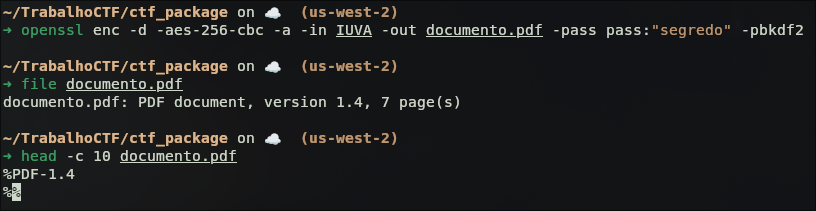
\includegraphics[width=1.0\textwidth]{screenshots/passo2_descriptografia.png}
    \caption{PDF descriptografado com sucesso - validação do header}
    \label{fig:passo2}
\end{figure}

\begin{figure}[H]
    \centering
    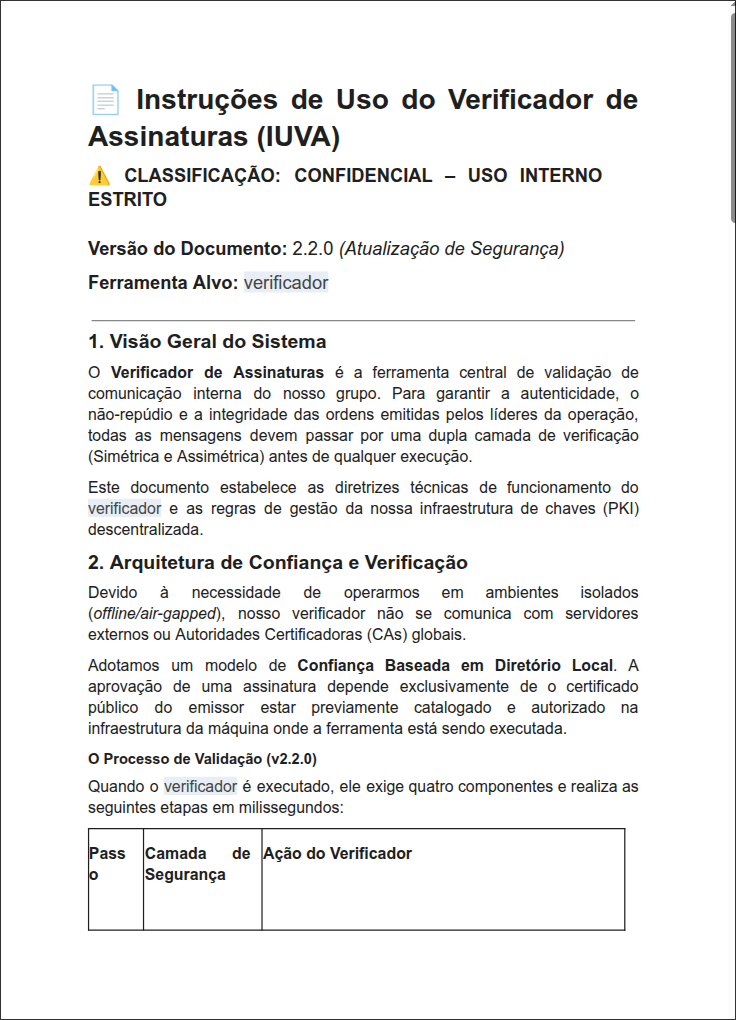
\includegraphics[width=1.0\textwidth]{screenshots/passo2_paginaInicial.png}
    \caption{Página inicial do PDF descriptografado}
    \label{fig:passo2_pagina}
\end{figure}

\subsection{Mapeamento de Primitivas Criptográficas}

Neste passo, a primitiva utilizada pelo sistema foi criptografia simétrica \texttt{AES-256-CBC} via OpenSSL.
O propósito arquitetural era preservar confidencialidade do documento IUVA.
A proteção não foi quebrada criptograficamente; o contorno ocorreu com uso legítimo da chave obtida no Passo 1 para realizar a operação de decriptação.


% ============================================================================
% PASSO 3: ANÁLISE DO VERIFICADOR
% ============================================================================

\section{Passo 3: Análise do Executável Verificador}

\subsection{Informações extraídas neste passo}

Com o conteúdo do PDF acessível, a próxima etapa é entender como o \texttt{verificador} decide se um documento e sua assinatura são confiáveis.
Os testes iniciais também mostraram que a ferramenta exige quatro entradas no fluxo final: mensagem, assinatura, certificado e HMAC-SHA256.

\subsection{Metodologia e Vetor de Ataque (Reprodutibilidade)}

\subsubsection{Comandos Utilizados}

\begin{lstlisting}[caption=Exploracao inicial do verificador]
file verificador
chmod +x verificador

# Executar para ver ajuda
./verificador

# Extrair strings interessantes
strings verificador | grep -i "usage\|verify\|sign\|key\|trust"

# Procurar por arquivos de chave/certificado
find . -name "*.pem" -o -name "*.key"

# Explorar trust store
ls -la .trust_store/
\end{lstlisting}

\subsubsection{Resultado observado e hipótese de vulnerabilidade}

\begin{figure}[H]
    \centering
    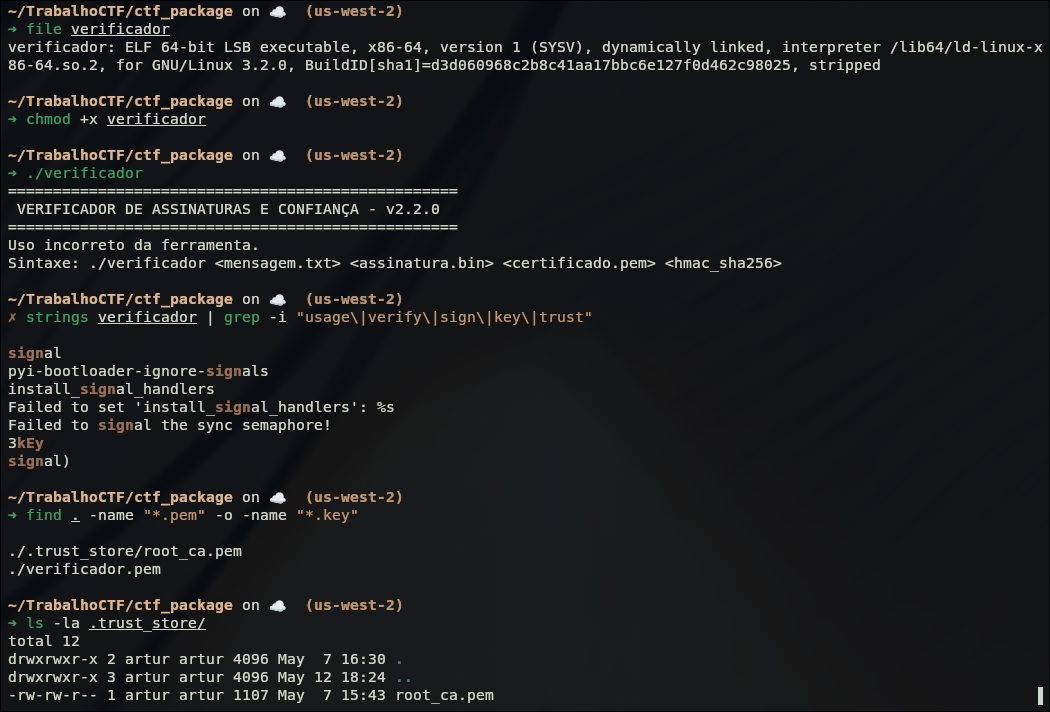
\includegraphics[width=1.0\textwidth]{screenshots/passo3_analise.png}
    \caption{Análise do verificador - saídas da etapa de reconhecimento}
    \label{fig:passo3}
\end{figure}

Hipótese de vulnerabilidade: o desenho de confiança parece estar concentrado no conteúdo local de \texttt{.trust\_store}. Se o verificador aceitar qualquer certificado encadeado (ou tratado como confiável) a partir desse diretório, então a inserção de um certificado forjado permite contornar a autenticação sem quebrar RSA. Além disso, a presença explícita de \texttt{<hmac\_sha256>} na sintaxe e strings internas relacionadas a segredo indicam que a proteção de integridade adicional depende de material embarcado no próprio binário.

Na fase de análise estática aprofundada, a constante de integridade utilizada pelo programa foi identificada como \texttt{1nt3gr1d4d3}, removendo a ambiguidade da pista inicial e permitindo reproduzir corretamente o cálculo do HMAC no Passo 7.

\subsection{Mapeamento de Primitivas Criptográficas}

Neste passo, não houve quebra direta de algoritmo criptográfico, e sim reconhecimento da arquitetura de confiança.
A análise mostrou dependência de artefatos de assinatura digital (RSA/SHA-256), certificados X.509 e um valor HMAC-SHA256 consumidos pelo verificador.
O contorno foi preparatório: identificar pontos de validação e os caminhos de trust store para, nos próximos passos, introduzir identidade forjada aceita pelo fluxo de verificação.


% ============================================================================
% PASSO 4: GERAÇÃO DE IDENTIDADE FORJADA
% ============================================================================

\section{Passo 4: Geração de Identidade Forjada}

\subsection{Informações extraídas neste passo}

A análise indica que, se conseguirmos introduzir uma identidade assinante dentro da confiança do sistema, o verificador tenderá a aceitar mensagens forjadas.

\subsection{Metodologia e Vetor de Ataque (Reprodutibilidade)}

\subsubsection{Comandos Utilizados}

\begin{lstlisting}[caption=Gerar chave privada e certificado]
# Gerar chave privada RSA
openssl genrsa -out admin_privada.pem 2048

# Gerar certificado autoassinado
openssl req -new -x509 -key admin_privada.pem \
  -out admin_certificado.pem -days 365 \
  -subj "/C=BR/ST=SC/L=Florianopolis/O=Infiltrado/CN=Admin"

# Verificar o certificado
openssl x509 -in admin_certificado.pem -text -noout
\end{lstlisting}

\subsubsection{Resultado observado}

\begin{figure}[H]
    \centering
    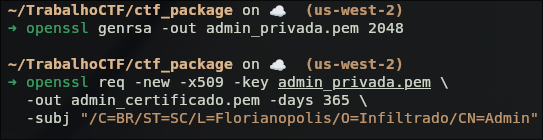
\includegraphics[width=1.0\textwidth]{screenshots/passo4_identidade.png}
    \caption{Execução da geração de chave e certificado forjado}
    \label{fig:passo4}
\end{figure}

\begin{figure}[H]
    \centering
    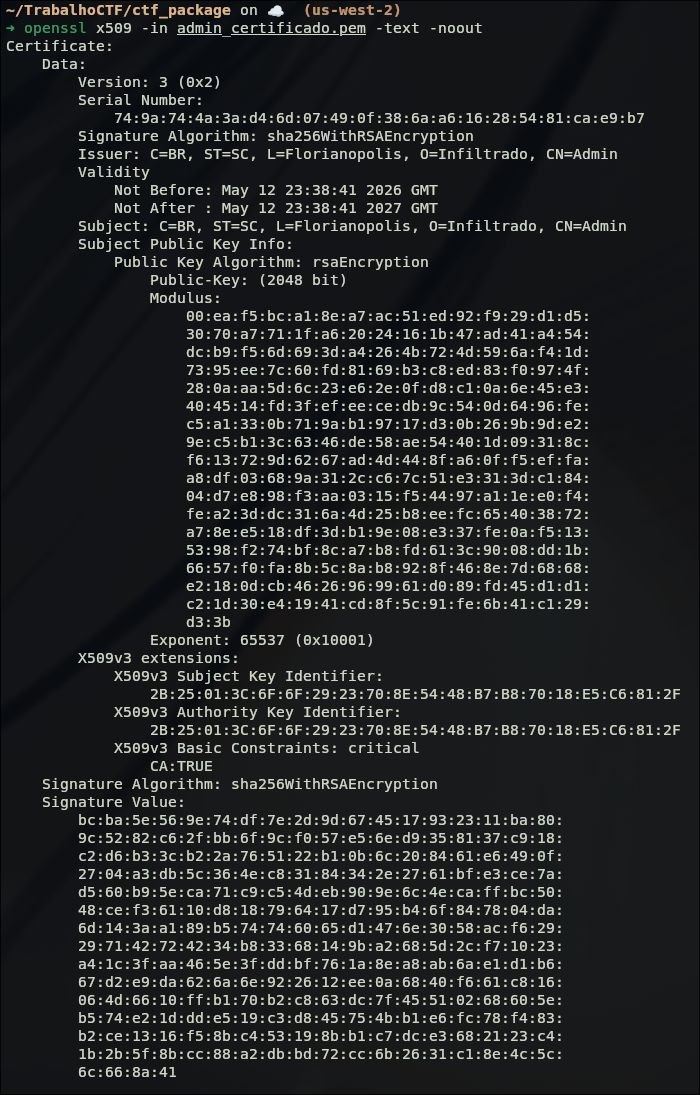
\includegraphics[width=1.0\textwidth]{screenshots/passo4_verificar_identidade.png}
    \caption{Verificação do certificado forjado}
    \label{fig:passo4_verificar}
\end{figure}

Foram criados dois arquivos principais: \textbf{admin\_privada.pem} (chave privada RSA-2048) e \textbf{admin\_certificado.pem} (certificado X.509 autoassinado com atributos administrativos).

\subsection{Mapeamento de Primitivas Criptográficas}

As primitivas deste passo foram criptografia assimétrica \texttt{RSA-2048} e certificado digital \texttt{X.509}.
O propósito arquitetural dessas primitivas é vincular uma identidade a uma chave pública confiável.
O contorno consistiu em gerar localmente um par de chaves e um certificado autoassinado com atributos administrativos, explorando a ausência de validação robusta da cadeia de certificação.


% ============================================================================
% PASSO 5: ASSINATURA DE DOCUMENTO
% ============================================================================

\section{Passo 5: Assinatura de Documento Forjado}

\subsection{Informações extraídas neste passo}

Com a identidade forjada criada, o próximo teste lógico é produzir um artefato assinado que possa ser submetido ao verificador.

\subsection{Metodologia e Vetor de Ataque (Reprodutibilidade)}

\subsubsection{Comandos Utilizados}

\begin{lstlisting}[caption=Criar e assinar documento]
# Criar documento de teste
cat > documento.txt << 'EOF'
ORDEM CONFIDENCIAL

De: Administrador do Sistema
Para: Agentes Operacionais
Assunto: Operacao em Andamento

Todos os agentes devem cumprir os protocolos.

Autorizado por: Administrador
EOF

# Assinar o documento
openssl dgst -sha256 -sign admin_privada.pem \
  documento.txt > documento.txt.sig

# Verificar tamanho da assinatura
ls -lh documento.txt.sig
\end{lstlisting}

\subsubsection{Resultado observado}

\begin{figure}[H]
    \centering
    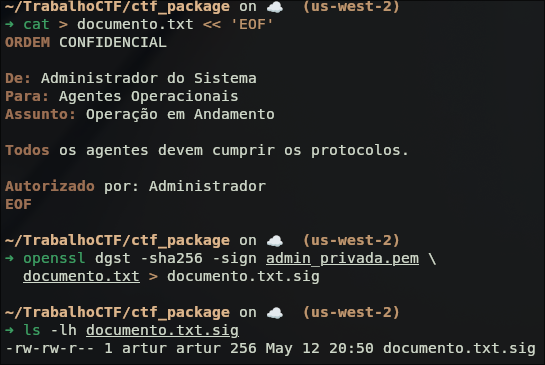
\includegraphics[width=1.0\textwidth]{screenshots/passo5_assinatura.png}
    \caption{Assinatura digital do documento forjado}
    \label{fig:passo5}
\end{figure}

A execução foi concluída sem erros e gerou o arquivo de assinatura \texttt{documento.txt.sig}.
O tamanho de \textbf{256 bytes} é compatível com assinatura \texttt{RSA-2048}, confirmando que o digest SHA-256 do documento foi assinado com sucesso pela chave privada forjada.

\subsection{Mapeamento de Primitivas Criptográficas}

As primitivas aplicadas foram função hash \texttt{SHA-256} e assinatura digital \texttt{RSA}.
O propósito arquitetural é garantir integridade e autenticidade do documento.
O contorno não exigiu quebra do algoritmo: a assinatura foi produzida corretamente, mas com uma chave privada forjada que o ambiente posteriormente aceita como confiável.

% ============================================================================
% PASSO 6: MANIPULAÇÃO DO TRUST STORE
% ============================================================================

\section{Passo 6: Manipulação do Trust Store}

\subsection{Informações extraídas neste passo}

A etapa crítica de exploração arquitetural é alterar o ponto de confiança local do sistema, isto é, o conteúdo do diretório \texttt{.trust\_store}.

\subsection{Metodologia e Vetor de Ataque (Reprodutibilidade)}

\subsubsection{Comandos Utilizados}

\begin{lstlisting}[caption=Adicionar certificado ao trust store]
cd ctf_package

# Copiar certificado para o trust store
cp admin_certificado.pem .trust_store/

# Listar conteudo do trust store
ls -la .trust_store/

# Verificar se foi adicionado
cat .trust_store/admin_certificado.pem | head -5
\end{lstlisting}

\subsubsection{Resultado observado}

\begin{figure}[H]
    \centering
    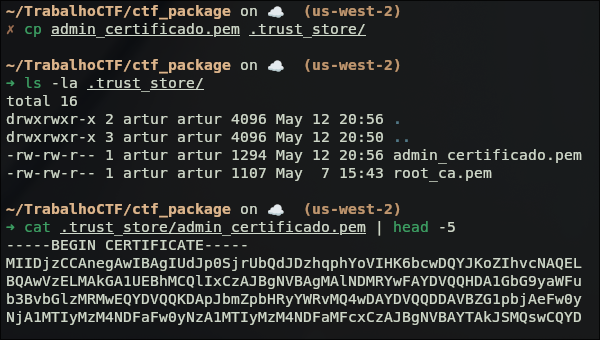
\includegraphics[width=1.0\textwidth]{screenshots/passo6_trust_store.png}
    \caption{Certificado forjado adicionado ao trust store}
    \label{fig:passo6}
\end{figure}

O certificado forjado foi copiado com sucesso para o diretório de confiança local por meio do comando \texttt{cp admin\_certificado.pem .trust\_store/}.

Na listagem do trust store, observou-se a presença simultânea do certificado forjado e da autoridade já existente:

\begin{lstlisting}
total 16
drwxrwxr-x 2 artur artur 4096 May 12 20:56 .
drwxrwxr-x 3 artur artur 4096 May 12 20:50 ..
-rw-rw-r-- 1 artur artur 1294 May 12 20:56 admin_certificado.pem
-rw-rw-r-- 1 artur artur 1107 May  7 15:43 root_ca.pem
\end{lstlisting}

A inspeção das primeiras linhas confirmou o formato PEM válido do arquivo inserido:

\begin{lstlisting}
-----BEGIN CERTIFICATE-----
MIIDjzCCAnegAwIBAgIUdJp0SjrUbQdJDzhqphYoVIHK6bcwDQYJKoZIhvcNAQEL
BQAwVzELMAkGA1UEBhMCQlIxCzAJBgNVBAgMAlNDMRYwFAYDVQQHDA1GbG9yaWFu
b3BvbGlzMRMwEQYDVQQKDApJbmZpbHRyYWRvMQ4wDAYDVQQDDAVBZG1pbjAeFw0y
NjA1MTIyMzM4NDFaFw0yNzA1MTIyMzM4NDFaMFcxCzAJBgNVBAYTAkJSMQswCQYD
\end{lstlisting}

Com isso, o trust store foi efetivamente alterado para incluir a identidade forjada como material confiável no processo de validação.

\subsection{Mapeamento de Primitivas Criptográficas}

Neste passo, o foco foi a primitiva de certificação X.509 no contexto de uma infraestrutura de confiança (PKI simplificada).
O propósito arquitetural era restringir validações apenas a emissores confiáveis.
O contorno ocorreu ao inserir manualmente o certificado forjado no \texttt{.trust\_store}, comprometendo a âncora de confiança utilizada pelo verificador.


% ============================================================================
% PASSO 7: APROVAÇÃO DO VERIFICADOR
% ============================================================================

\section{Passo 7: Teste Final - Aprovação do Verificador}

\subsection{Informações extraídas neste passo}

Após comprometer o trust store, resta validar se o fluxo de verificação aceita, na prática, uma assinatura produzida com identidade forjada.

\subsection{Metodologia e Vetor de Ataque (Reprodutibilidade)}

\subsubsection{Comandos Utilizados}

\begin{lstlisting}[caption=Testar com o verificador]
# Gerar HMAC-SHA256 esperado pelo verificador
HMAC=$(openssl dgst -sha256 -hmac '1nt3gr1d4d3' documento.txt | awk '{print $NF}')

# Executar o verificador com os 4 argumentos corretos
./verificador documento.txt documento.txt.sig admin_certificado.pem "$HMAC"
\end{lstlisting}

\subsubsection{Resultado observado}

\begin{figure}[H]
    \centering
    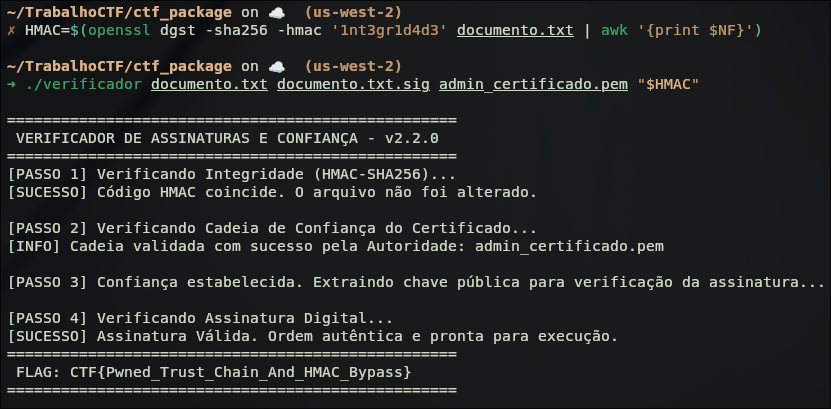
\includegraphics[width=1.0\textwidth]{screenshots/passo7_aprovacao.png}
    \caption{\textbf{EVIDÊNCIA CRÍTICA}: O verificador aprova o documento forjado}
    \label{fig:passo7}
\end{figure}

Esse resultado confirma, na prática, que o documento forjado foi aceito pelo mecanismo de verificação após o comprometimento da cadeia de confiança e o fornecimento do código de integridade esperado.

Para fins de reprodutibilidade textual (além da captura de tela), o terminal apresentou, de forma resumida:

\begin{lstlisting}
[PASSO 1] Verificando Integridade (HMAC-SHA256)... [SUCESSO]
[PASSO 2] Verificando Cadeia de Confianca do Certificado... [SUCESSO]
[PASSO 4] Verificando Assinatura Digital... [SUCESSO]
FLAG: CTF{Pwned_Trust_Chain_And_HMAC_Bypass}
\end{lstlisting}

\subsection{Mapeamento de Primitivas Criptográficas}

Na etapa final, o verificador combina assinatura digital (RSA + SHA-256) com validação de cadeia de confiança X.509.
O propósito arquitetural desse desenho é aceitar somente documentos assinados por identidades autênticas e confiáveis.
O contorno foi efetivo porque a cadeia de confiança já estava comprometida: a assinatura forjada passa na verificação por ter sido emitida por certificado inserido no trust store do próprio sistema.

% ============================================================================
% RECOMENDAÇÕES
% ============================================================================

\section{Recomendações de Mitigação}

Com base nas etapas exploradas, as seguintes medidas reduzem significativamente a superfície de ataque observada:

\begin{itemize}
    \item Remover segredos de integridade hardcoded no cliente e migrar a validação de HMAC para contexto server-side ou para mecanismo com proteção de segredo em hardware.
    \item Proteger o trust store contra escrita por usuários não privilegiados, incluindo permissões restritivas e validação de cadeia com pinning da CA raiz esperada.
    \item Exigir validação estrita de certificado (cadeia completa, emissor esperado, período de validade e constraints de uso) antes da verificação da assinatura.
    \item Implementar trilhas de auditoria e alertas para alterações em \texttt{.trust\_store} e para tentativas de validação com novos certificados.
\end{itemize}

% ============================================================================
% CONCLUSÃO
% ============================================================================

\section{Conclusão Técnica}

O fluxo reproduzido demonstra uma falha arquitetural de confiança e não uma quebra matemática das primitivas criptográficas.

Em sequência, foi possível: recuperar informação-chave no \texttt{secret.txt}, decriptar o conteúdo protegido com \texttt{AES-256-CBC}, entender a lógica do \texttt{verificador}, produzir identidade e assinatura forjadas com \texttt{RSA/X.509}, comprometer o \texttt{.trust\_store} e obter aprovação final do artefato forjado.

As evidências visuais permanecem distribuídas ao longo das sessões de Passo 1 a Passo 7, acompanhando cada etapa no momento em que foi executada, como um registro técnico contínuo da operação.

Com o sucesso do ataque, o impacto observado foi:

\begin{itemize}
    \item Descriptografar dados confidenciais
    \item Forjar identidades aceitas pelo sistema
    \item Assinar documentos como autoridades do sistema
    \item Infiltrar-se completamente na infraestrutura
\end{itemize}

\textbf{Conclusão:} O sistema foi completamente comprometido.

\end{document}
